\documentclass[14pt]{article}
\usepackage{graphicx}

\usepackage{multirow}
\usepackage{verse}
\newcommand{\attrib}[1]{%
\nopagebreak{\raggedright\footnotesize #1\par}}
\renewcommand{\poemtitlefont}{\normalfont\large\itshape\centering}
 
\usepackage{chemfig}
\usepackage{circuitikz}
\usepackage{amsmath}

\usepackage{pgfplots}
\pgfplotsset{width=7cm,compat=1.8}

\usepackage{geometry}

\usepackage[%
  newcommands     % \RaggedRight=\raggedright etc. 
 ,newparameters   % use default settings of ragged2e
]{ragged2e}
\usepackage[pdfauthor={Sina Ahmadi},
            pdftitle={XeLaTeX ژ بۆ نڤیساندنا ب کوردی}]{hyperref}
            
\hypersetup{colorlinks,breaklinks,
            urlcolor=[rgb]{0,0.5,0.5},
            linkcolor=[rgb]{0,0.5,0.5}}

\usepackage{listings}
\lstset{%
language={[LaTeX]TeX},
numbersep=5mm,
basicstyle=\footnotesize,
numbers=left,
stepnumber=1,
numberstyle=\tiny,
breaklines=true,frame=single,framexleftmargin=2mm, xleftmargin=2mm,
prebreak = \raisebox{0ex}[0ex][0ex]{\ensuremath{\hookleftarrow}},
backgroundcolor=\color{green!5},frameround=fttt,escapeinside=??,
rulecolor=\color{red},
morekeywords={
    maketitle},
keywordstyle=\color[rgb]{0,0,1},                    
        commentstyle=\color[rgb]{0.133,0.545,0.133},
        stringstyle=\color[rgb]{0.627,0.126,0.941}
}
% numerals: eastern and western

% numerals: eastern and western

\usepackage{polyglossia}
\setdefaultlanguage[variant=Kurmanji,script=Arabic,numerals=eastern]{kurdish} 
\newfontfamily\arabicfont[Script=Arabic,Scale=1]{Yas}
\newfontfamily\greekfont{Times New Roman}[Script=Greek]
\let\arabicfonttt\ttfamily
\setotherlanguage{english}
\setotherlanguage[variant=poly]{greek}


\title{\textenglish{\XeLaTeX} ژ بۆ نڤیساندنا ب کوردی}
\author{سینا ئەحمەدی \\ {\small \url{https://sinaahmadi.github.io/}}}
\date{\today}

\begin{document}

\maketitle
\tableofcontents

\begin{abstract}
ئەڤ دەمەک بوویە کو من دخوەست کو ژ بۆ نڤیساندنا ب کوردی سیستەما نڤیسا 
\textenglish{\TeX}
 ب کاربینم. ئەڤ ژ من رە تەشویق کر کو من ئەو ل سەر پاکێتا 
\texttt{\textenglish{Polyglossia}}
 زێدە بکم. د ڤەرسییۆنا نھا دە، زاراڤایێن سۆرانی و کورمانجی ب دو رێنڤیسێن عەرەبی و لاتینی رە ھەنە. ئەڤ بەلگە ب کورتی ئاگاھداری ددە کو بەلگەیێن خوە ب کوردی ب 
 \textenglish{\XeLaTeX}
   بافرینن \footnote{نڤیسکار ب سۆرانی داخڤە. ژ کەرەما خوە ببەخشینە ئەگەر نڤیساندنا وی ب کورمانجی نە پڕ باشە.}.
   ژ بۆ زێدەتر ئاگاھداری، بچن
   \textenglish{\url{https://kurdishxelatex.github.io/}}.
\end{abstract}



\section{\textenglish{\TeX} چی یە؟}

\textenglish{\TeX}
 سیستەما ئامادە کرنا نڤیسێ ((\textenglish{typesetting})  ب ئینگلیسی) یە کو "ژ بۆ ئافراندنا پرتووکێن خوەشک و ب تایبەتی ژ بۆ پرتووکێن کو گەلەک ماتەماتیکێ تێ دە ھەیە" یە \cite{knuth1984texbook}. بەرەڤاژی سیستەمێن دن ئێن پرۆسە کرنا نڤیسان، مینا 
 \textenglish{Microsoft Office} 
 کو
\textenglish{\textit{what you see is what you get}}
\footnote{ب کوردی، "یا کو ھوون دبینن، تشتێ کو ھوون دگرنە"}
   ب کار تینن، نڤیساندنا ل سەر 
 \textenglish{\TeX}
   ب ب کارانینا نڤیسا سادە ل گۆری سنتاکسیا 
 \textenglish{\TeX}
    پێک تێ.
 \textenglish{\TeX} 
     د سالا ١٩٧٨-ان دە ژ ھێلا زانیارێ کۆمپیوتر، دۆنالد کنوت ڤە ھات چێکرن. ئارمانجا سەرەکەیا 
 \textenglish{\TeX}
      ئالیکاریا کارووبارێ نڤیساندنێ یە. نڤیسکاران دڤێ خوەدان ئامووران بە ژ بۆ نڤیساندنێ ھەمی تشتێ کو دخوازن، ھەلبەست بە، ھەڤسەنگییەک کیمیەوی بە ئان فۆرمولەک ماتەماتیکی. گۆتنا 
 \textenglish{\TeX} 
       ژ پەیڤا یەونانی
 \textgreek{\textit{τέχνη}} 
       یە کو تێ واتەیا ھونەرێ. ژ بەر کو فۆنەما
 \textgreek{χ} 
       د کوردی دە (و گەلەک زمانێن دن) تونە یە، ئەم دکارن ببێژن تێک ئان تێخ، لێ نە تێکس!


ھن تایبەتمەندیێن سەرەکە یێن 
 \textenglish{\TeX}
  وەکێ ژێرینن:
\begin{itemize}
\item   ئامادە کرنا کۆڤار، پرتووک، راپۆرت، گۆتار و سلایدێن پێشکێشی
\item   بەلگەیێن مەزن ب گەلەک بەش و داباشان رە خستن
\item   نڤیساندنا ماتەماتیکێ و زانستێن دن و مژارێن تەکنیکی
\item   ساز کرنا بیبلیۆگرافی و رەفەرانس دان ب ھێسانی
\item   ب کار ئانینا ھێژایا ماتەریالێ گرافیکی
\item   ڤەگوھەزتنا فۆرماتێن دنێن مینا HTML
\end{itemize}

د بنگەھا 
\textenglish{\TeX} 
 دە، گەلەک سیستەمەک دن ھاتنە ئافراندن ژ بۆ پشتگریا زمان و نڤیسارێن دن. 
 \textenglish{\LaTeX} 
  و 
 \textenglish{\XeLaTeX} 
   دو سیستەمێن بەرناسن کو ئیرۆ ب بەرفرەھی تێنە بکار ئانین.


\section{\XeLaTeX~ژ بۆ کوردی}

بەلگەیەک سادە د 
 \textenglish{\LaTeX} 
 دە د دیمەنێ
 \ref{fig_mwe}  
 دە تێ نیشاندان. وەکی کو ھوون دبینن، ئەم دیار ناکن جھێ کو سەرناڤێ دەردکەڤە ئان تاریخ ب چ فۆرمەک بە. سیستەمێ 
 \textenglish{\TeX} 
  خوە بریار ددە چاوا بەلگەیەک چێ ببە.

\begin{figure}[h]
    \centering
    \begin{minipage}{0.29\textwidth}
        \fbox{
               \centering
        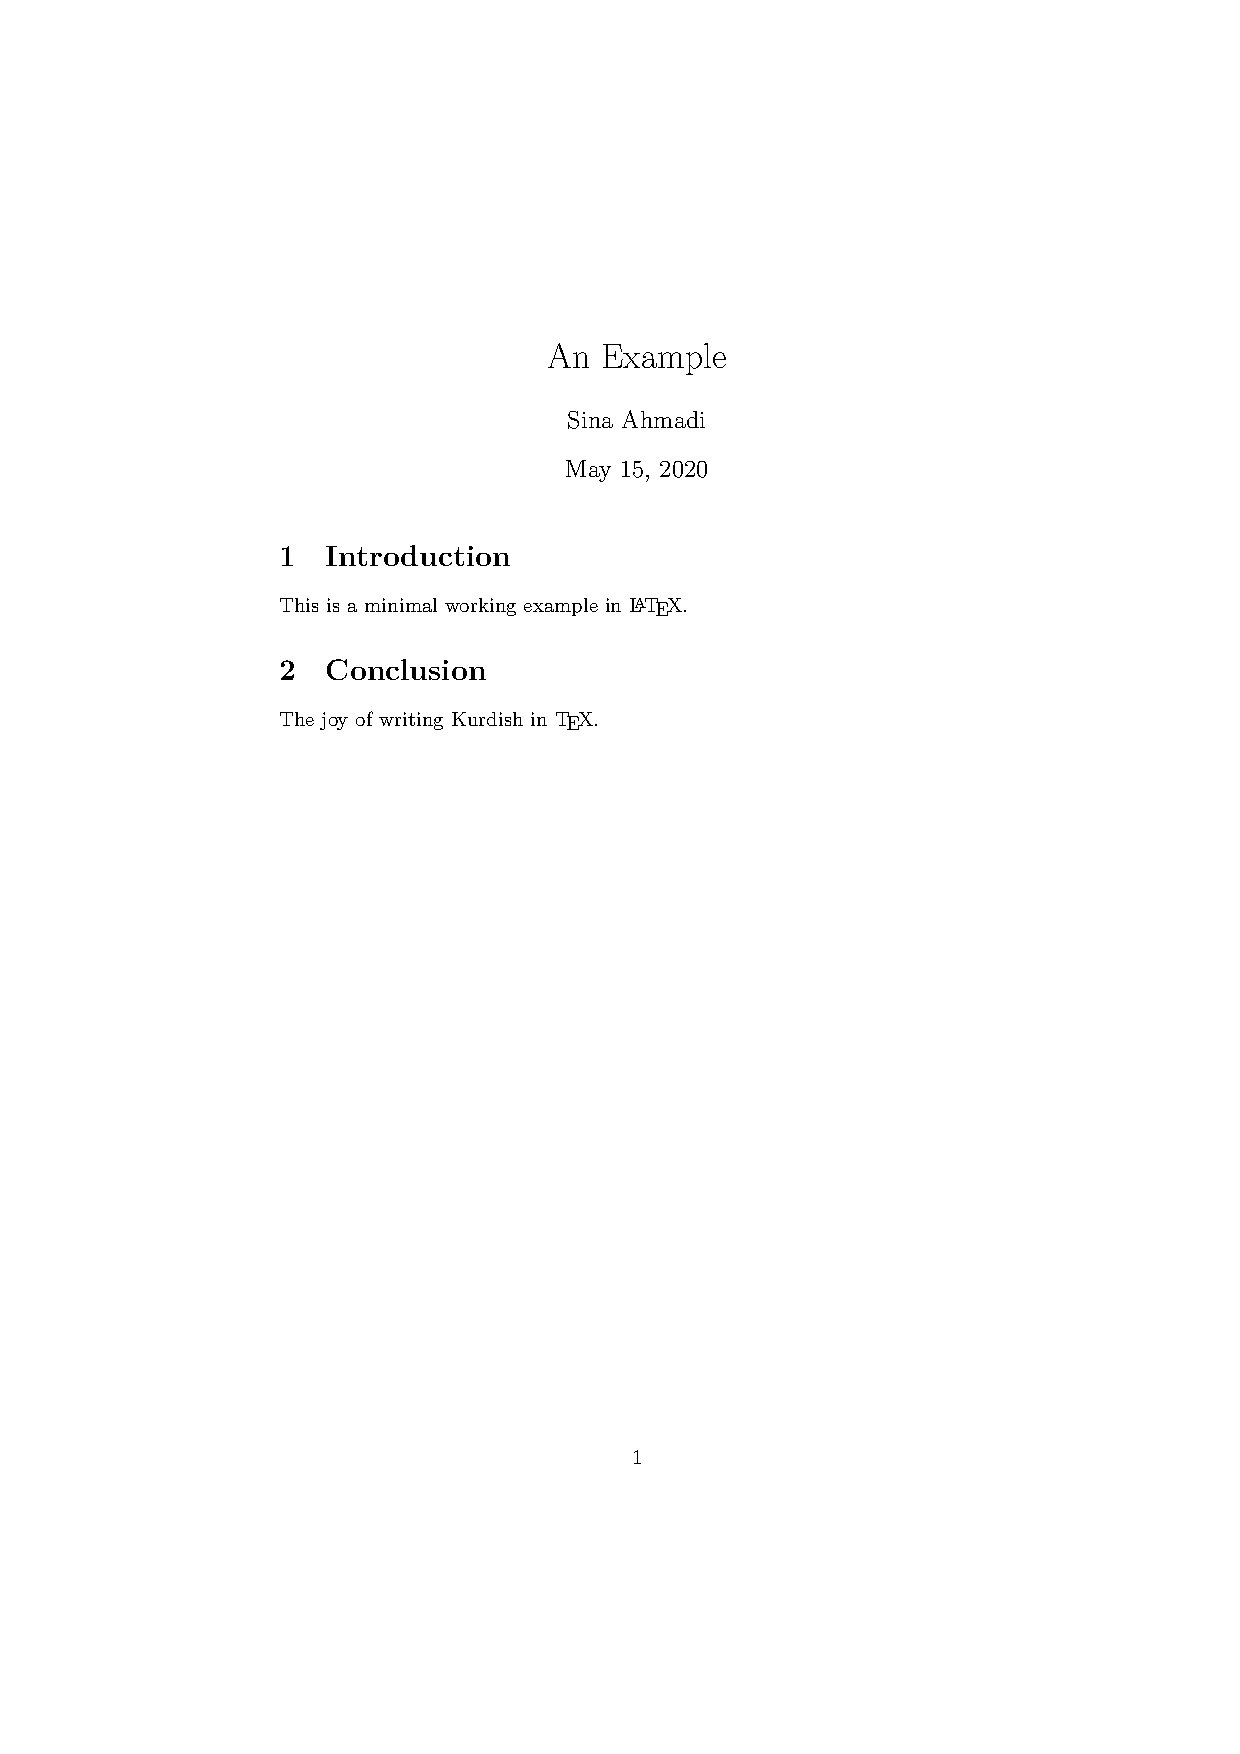
\includegraphics[width=\textwidth]{figure_example.pdf} 
        }
    \end{minipage}\hfill
    \begin{minipage}{0.65\textwidth}
\begin{english}
\begin{lstlisting}
\documentclass{article}
\usepackage[utf8]{inputenc}

\title{An Example}
\author{Sina Ahmadi}
\date{\today}

\begin{document}

\maketitle
\section{Introduction}

This is a minimal working example in \LaTeX.

\section{Conclusion}

The joy of writing Kurdish in \TeX.

\end{document}

\end{lstlisting}
\end{english}
    \end{minipage}
 \caption{نموونەیەک ل بەلگەیەک کو ب \LaTeX~ ھاتیە نڤیسین. ل ملێ چەپێ، کۆدێ بەلگەیێیە و ل ملێ راستێ ژی ئاکامێ کامپایل کرنێیە}
 \label{fig_mwe}
\end{figure}

بەرێ، 
\textenglish{\TeX} 
 تەنێ چەند زمانان ب تیپێن لاتینی پشتگری دکر و پشترا، گەلەک زمان و نڤیسار ھاتن زێدە کرن. 
  \textenglish{\XeLaTeX} 
  ل سەر 
 \textenglish{\TeX} 
   ھاتە ئافراندن و ل یوونیکۆد پشتگری دکە. کوردی گەلەک زاراڤ و نڤیسێن وی ھەنە و 
 \textenglish{\XeLaTeX}    
    ژ بۆ وی سیستەمەک ئیدەالە، ب تایبەتی ب 
\texttt{\textenglish{Polyglossia}}\footnote{\url{https://github.com/reutenauer/polyglossia}}
    . ژ بۆ ئافراندنا بەلگەیەک ب 
 \textenglish{\XeLaTeX}   
     ب کوردی، دڤێ بەلگەیا وە وھا بە:


\begin{english}
\begin{lstlisting}
  \documentclass{article}
  \usepackage{polyglossia}
  \setmainfont{Times New Roman}
  \setdefaultlanguage[variant=sorani,script=latin,numerals=western]{kurdish}

  \title{Nûsrawekeyekî Min}
  \author{Nawî min}
  \date{\ontoday}

  \begin{document}

  \maketitle

  \end{document}
\end{lstlisting}
\end{english}

د رێزا یەکەم دە، ھوون دبێژن کو بەلگەیا وە گۆتارەکە (\textenglish{article} ). رێزێن ٢ ھەتا ٤ ژ بۆ ب کارانینا \texttt{\textenglish{Polyglossia}}
یە و دبێژن کو دخوازن کورمانجی ب رێنڤیسا لاتینی ب کار بینن. کەڤالا 
\ref{tab_polyglot_options}
سەرجەم ڤەبژارکێن 
\texttt{\textenglish{Polyglossia}}
 ژ بۆ کوردی نیشان ددە.
 
 
\begin{table}[h]
\centering
\begin{english}
\begin{tabular}{l|l|l|l} 
 \hline
Polyglossia         & variant  & script        & numerals         \\ \hline \hline
\multirow{2}{*}{Kurdish} & \texttt{sorani}   & \texttt{arabic}, \texttt{latin} & \texttt{eastern}, \texttt{western} \\  \cline{2-4} 
                         & \texttt{kurmanji} & \texttt{arabic}, \texttt{latin} & \texttt{eastern}, \texttt{western} \\ \hline
\end{tabular}
\end{english}
\caption{ڤەبژارکێن \texttt{\textenglish{Polyglossia}} ژ بۆ ئافراندنا بەلگەیەک ب کوردی}
\label{tab_polyglot_options}
\end{table}

بۆ نموونە، گەر ھوون دخوازن ب سۆرانی ب ھەژمارەک تیپێن عەرەبی و رێنڤیسا عەرەبی بەلگەیەک چێبکن، ھوون میھەنگێن خوە ل رێزا ٤ وھا دگوھەزن:


\begin{english}
\begin{lstlisting}
 \setdefaultlanguage[variant=sorani,script=arabic,numerals=eastern]{kurdish}
\end{lstlisting}
\end{english}

د دەربارێ سالنامەیێ دە، ل ڤەرسییۆنا نھا ژ 
\texttt{\textenglish{Polyglossia}}
 سالنامەیا زایینی ب تەنێ ھەیە.
 کەڤالا
\ref{tab_polyglot_options}
 ناڤێن مەھان ل ھەمی میھەنگان نیشان ددە. بالا خوە بدن کو دو رەوشان ھەنە ژ بۆ نیشاندانا تاریخێ:
\texttt{\textenglish{\textbackslash today}}
و
\texttt{\textenglish{\textbackslash ontoday}}. 
 ل رەوشێ یەکەم دە، تەنێ ناڤێ مەھا و ھەژمارێن رۆژ و سال تێ، بۆنموونە، ٣٠ گولان ٢٠٢٠. لێ ل رەوشێ پاشین، 
 "\textenglish{î/y}" یا
  ئیزافە ژی تێ، بۆ نموونە ٣٠ێ گولانێ ٢٠٢٠.
ڤێ ڤەبژارکێ تەنێ دەما کارانینا تیپێن لاتینی پەیدا دبە.

\begin{table}[!h]
\centering
\begin{english}
\begin{tabular}{|l|l|l|l|l|} 
\hline
{\arabicfont{ئینگلیسی}} & {\arabicfont{عەرەبی - سۆرانی}} & {\arabicfont{ لاتینی - سۆرانی}} & {\arabicfont{عەرەبی - کرمانجی}} & {\arabicfont{لاتینی - کرمانجی}} \\\hline\hline
January & {\arabicfont{ دووهەم كانوونی}} & Kanûnî Dûhem & {\arabicfont{پاشین  چلەیا}} & Çileya Paşîn \\ 
February & {\arabicfont{شوبات}} & Şubat & {\arabicfont{شبات }} & Sibat \\
March & {\arabicfont{ ئازار }} & Azar & {\arabicfont{ ئادار }} & Adar \\
April & {\arabicfont{نیسان }} & Nîsan & {\arabicfont{ نیسان }} & Nîsan \\
May & {\arabicfont{ئایار }} & Ayar & {\arabicfont{ گولان }} & Gulan \\
June & {\arabicfont{حوزەیران }} & Huzeyran & {\arabicfont{ حەزیران }} & Hezîran \\
July & {\arabicfont{ تەممووز }} & Temmûz & {\arabicfont{ تیرمەهـ }} & Tîrmeh \\
August & {\arabicfont{ ئاب }} & Ab & {\arabicfont{ تەباخ }} & Tebax \\
September & {\arabicfont{ئەیلوول }} & Eylûl & {\arabicfont{ ئیلۆن }} & Îlon \\
October & {\arabicfont{  یەكەم تشرینی}} & Tişrînî Yekem & {\arabicfont{  پێشین چریا  }} & Çiriya Pêşîn \\
November & {\arabicfont{  دووهەم تشرینی}} & Tişrînî Dûhem & {\arabicfont{ پاشین چریا }} & Çiriya Paşîn \\
December & {\arabicfont{  یەكەم كانوونی}} & Kanûnî Yekem & {\arabicfont{پێشین چلەیا  }} & Çileya Pêşîn \\ \hline
\end{tabular}
\end{english}
\caption{نێوی مانگەکان لە \texttt{\textenglish{Polyglossia}}دا}
\label{tab_polyglot_calendar}
\end{table}

ژ بۆ زانیارییا زێدەتر ل سەرپۆلیگلۆسساوو زمانێ کوردی، ل
\cite{Charette2020} و \cite{ahmadi2020TexforKurdish} 
بنهێرن.


\section{چەند نموونەیان ب \texttt{\textenglish{Polyglossia}} }

\subsection{\XeLaTeX~ بۆ وێژە و هونەر}

\poemtitle*{یادگاری شیرن}
\settowidth{\versewidth}{چاوەکەم! چاوی ڕەشی تۆ ئافەتی گیانی منە}
\begin{verse}[\versewidth]
چاوەکەم! چاوی ڕەشی تۆ ئافەتی گیانی منە \\
گیانەکەم! برژانگی تیژت نووکە ڕمبی دوژمنە \\
 \vin شیری دەستی شێری ئاڵایە برۆ راکشاوەکەت \\
\vin جەرگی لاوێکی هەژاری کوردی ورد پێ بنجنە \\ 
چۆن دەبێ سەربەست گەلی ژێردەست کە کچ دابەستە بێ؟ \\
بەس نەبێ ئەو کۆیلەتی و ئەو کچ لە ژوور دابەستنە \\
\vin دەرکی داخستووە لە تۆ بابت کەچی دەرکی نییە \\
\vin دەرکە داخستن لە تۆ دەرکی هومێد داخستنە \\
\end{verse}
\attrib{لە دیوانی مامۆستا هێمن}


\subsection{\XeLaTeX~ بۆ زانست و بیرکاری}

\begin{center}
\setchemfig{atom sep=2em,bond style={line width=1pt,red,dash pattern=on 2pt off 2pt}}  
\chemname
{\chemfig{H-C(-[2]H)(-[6]H)-C(=[1]O)-[7]H}}
{ئێتانال (Ethanal)}
\end{center}


\begin{equation}\label{equation_example}
  x = a_0 + \frac{1}{\displaystyle a_1 
          + \frac{1}{\displaystyle a_2 
          + \frac{1}{\displaystyle a_3 + a_4}}}
\end{equation}


\begin{figure}[h]
\centering
\begin{minipage}[b]{.48\textwidth}
% source of the following: https://www.overleaf.com/learn/latex/CircuiTikz_package
\begin{circuitikz}[american voltages]
\draw
  (0,0) to [short, *-] (6,0)
  to [V, l_=$\mathrm{j}{\omega}_m \underline{\psi}^s_R$] (6,2) 
  to [R, l_=$R_R$] (6,4) 
  to [short, i_=$\underline{i}^s_R$] (5,4) 
  (0,0) to [open, v^>=$\underline{u}^s_s$] (0,4) 
  to [short, *- ,i=$\underline{i}^s_s$] (1,4) 
  to [R, l=$R_s$] (3,4)
  to [L, l=$L_{\sigma}$] (5,4) 
  to [short, i_=$\underline{i}^s_M$] (5,3) 
  to [L, l_=$L_M$] (5,0); 
  \end{circuitikz}
\caption{سێرکت بۆ نموونە}
\label{example_circuit}
\end{minipage}\hfill
\begin{minipage}[b]{.4\textwidth}
  \centering
\begin{tikzpicture}
\begin{axis}[
    title={$x \exp(-x^2-y^2)$}, 
    xlabel=$x$, ylabel=$y$,
	small,
]
\addplot3[
	surf,
	domain=-2:2,
	domain y=-1.3:1.3,
] 
	{exp(-x^2-y^2)*x};
\end{axis}
\end{tikzpicture}
\caption{فانکشنێکی ماتماتیک}
\label{example_function}
\end{minipage}
\end{figure}

\section{ئەنجام}
د ڤێ گۆتارێ دە، مە ب کورتاھی نیقاش کر چاوا 
\XeLaTeX~
 ب پاکێتا
 \texttt{Polyglossia}
ژ بۆ نڤیساندناب کوردی رە بکار تینە. ژ بۆ زانیارییا زێدەتر، بچن 
\href{https://kurdishxelatex.github.io/}{کۆما بکارینەرێن \XeLaTeX~یا کوردی}
. ھوون دکارن ژ ھێلا ئافراندنا ناڤەرۆکێ ژی بەشداری ڤێ کۆمێ ببن.

\bibliographystyle{unsrt}
\bibliography{bibliography}

\end{document}
